% Created 2024-04-04 Thu 13:21
% Intended LaTeX compiler: pdflatex
\documentclass[11pt]{article}
\usepackage[utf8]{inputenc}
\usepackage[T1]{fontenc}
\usepackage{graphicx}
\usepackage{longtable}
\usepackage{wrapfig}
\usepackage{rotating}
\usepackage[normalem]{ulem}
\usepackage{amsmath}
\usepackage{amssymb}
\usepackage{capt-of}
\usepackage{hyperref}
\usepackage{listings}
\usepackage{color}
\usepackage{amsmath}
\usepackage{array}
\usepackage[T1]{fontenc}
\usepackage{natbib}
\author{Anders Munch}
\date{\today}
\title{statelearner sim results}
\begin{document}

\maketitle
\tableofcontents

n\#+OPTIONS:   num:t toc:nil ':t \^{}:t

\section{IPCW super learners}
\label{sec:org30b08e8}

\begin{verbatim}
     n_obs    sim_set  type            SL time type.1       IPA           se
  1:   300   original  cens        survSL    6   cens 0.6978450 0.0008305614
  2:   300   original  cens State learner    6   cens 0.6989384 0.0008192387
  3:   300   original  cens        Oracle    6   cens 0.6992857 0.0008149009
  4:   300   original event        survSL    6  event 0.3488385 0.0019823097
  5:   300   original event State learner    6  event 0.3468667 0.0019972122
 ---                                                                        
380:  2400 indep_cens event        survSL   36  event 0.1922440 0.0003727166
381:  2400 indep_cens event State learner   36  event 0.2005905 0.0002755740
382:  2400 indep_cens event      IPCW(KM)   36  event 0.2005905 0.0002755740
383:  2400 indep_cens event     IPCW(Cox)   36  event 0.2005905 0.0002755740
384:  2400 indep_cens event        Oracle   36  event 0.2005905 0.0002755740
     n_obs               sim_set  type            SL time type.1       IPA           se
  1:   300   Dependent censoring  cens        survSL    6   cens 0.6978450 0.0008305614
  2:   300   Dependent censoring  cens State learner    6   cens 0.6989384 0.0008192387
  3:   300   Dependent censoring  cens        Oracle    6   cens 0.6992857 0.0008149009
  4:   300   Dependent censoring event        survSL    6  event 0.3488385 0.0019823097
  5:   300   Dependent censoring event State learner    6  event 0.3468667 0.0019972122
 ---                                                                                   
380:  2400 Independent censoring event        survSL   36  event 0.1922440 0.0003727166
381:  2400 Independent censoring event State learner   36  event 0.2005905 0.0002755740
382:  2400 Independent censoring event      IPCW(KM)   36  event 0.2005905 0.0002755740
383:  2400 Independent censoring event     IPCW(Cox)   36  event 0.2005905 0.0002755740
384:  2400 Independent censoring event        Oracle   36  event 0.2005905 0.0002755740
\end{verbatim}

\begin{center}
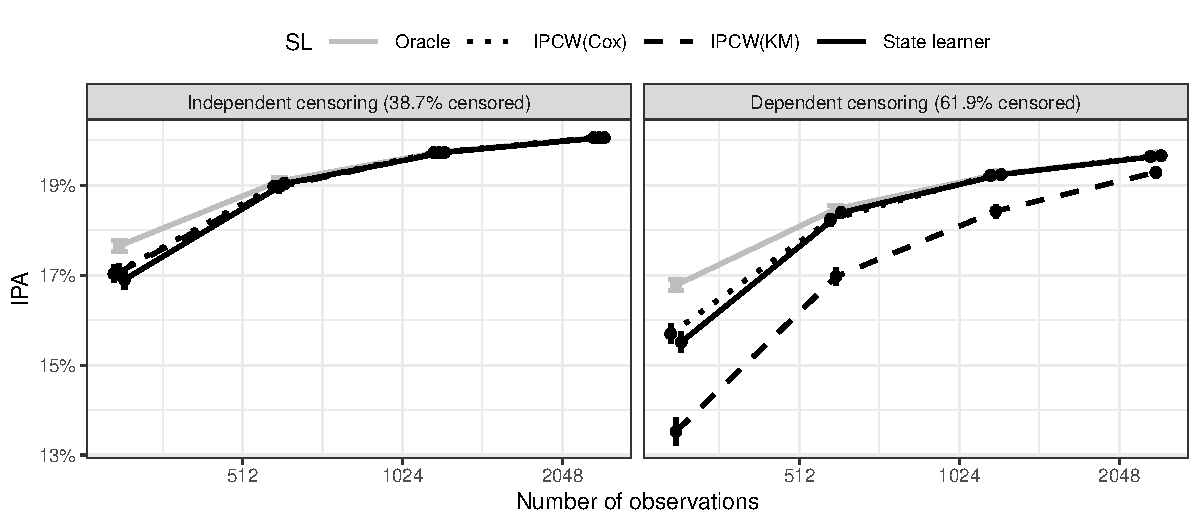
\includegraphics[width=.9\linewidth]{experiment-fig-sl-ipcw.pdf}
\end{center}

\section{survSL}
\label{sec:org8951f83}
\begin{center}
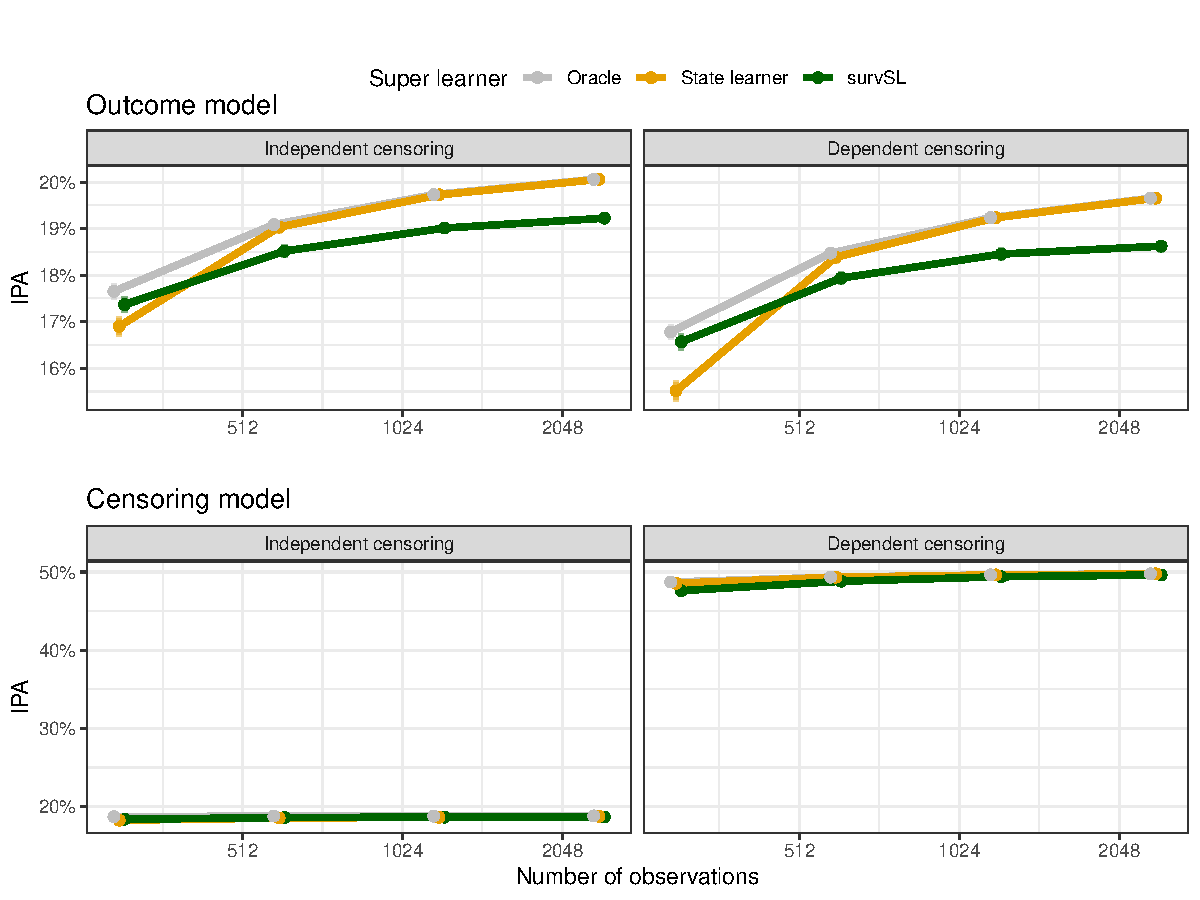
\includegraphics[width=.9\linewidth]{experiment-fig-sl-survSL.pdf}
\end{center}


\section{Real Zelefski data with competing event new version}
\label{sec:org1137d4f}

\subsection{State learner}
\label{sec:orgec9334e}
\begin{center}
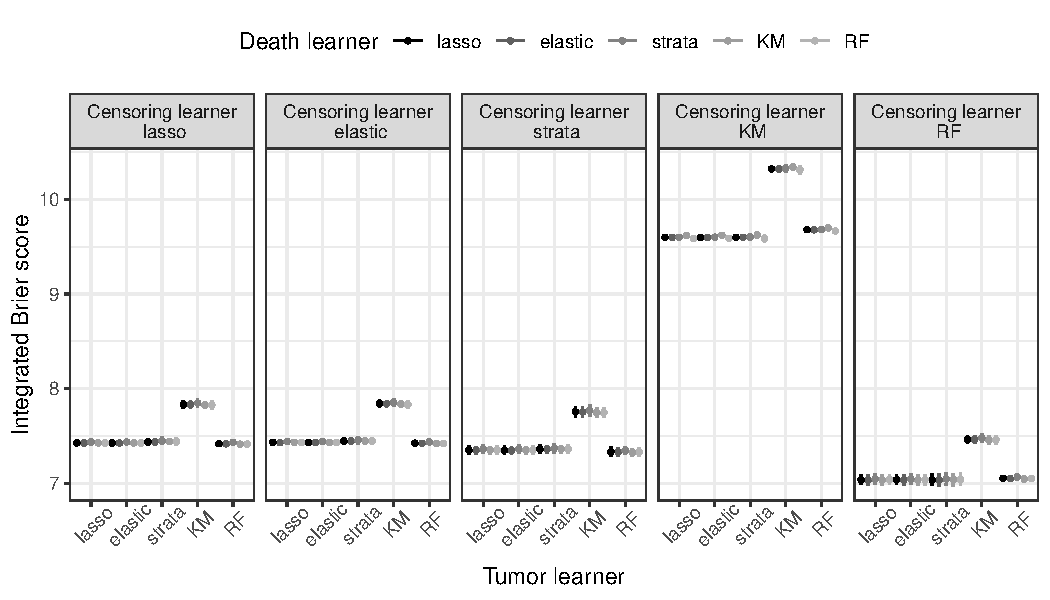
\includegraphics[width=.9\linewidth]{zelefski-real-data.pdf}
\end{center}

Table

\begin{verbatim}
                      cause1           cause2 censor      loss          sd
  1:            \\texttt{RF}               km     rf  7.022057 0.046024265
  2: \\texttt{Cox strata CT}      cox_elastic     rf  7.025097 0.032110343
  3:            \\texttt{RF}      cox_elastic     rf  7.025267 0.046638952
  4:            \\texttt{RF}               rf     rf  7.025504 0.046457079
  5: \\texttt{Cox strata CT}        cox_lasso     rf  7.025648 0.031585447
 ---                                                                      
121:            \\texttt{KM}               rf     km 10.299304 0.005481968
122:            \\texttt{KM}        cox_lasso     km 10.310004 0.004864230
123:            \\texttt{KM}      cox_elastic     km 10.310062 0.005185197
124:            \\texttt{KM} cox_strata_stage     km 10.310763 0.003174509
125:            \\texttt{KM}               km     km 10.328653 0.004108411
                      cause1                  cause2 censor      loss          sd
  1:            \\texttt{RF}            \\texttt{KM}     rf  7.022057 0.046024265
  2: \\texttt{Cox strata CT}       \\texttt{Elastic}     rf  7.025097 0.032110343
  3:            \\texttt{RF}       \\texttt{Elastic}     rf  7.025267 0.046638952
  4:            \\texttt{RF}            \\texttt{RF}     rf  7.025504 0.046457079
  5: \\texttt{Cox strata CT}         \\texttt{Lasso}     rf  7.025648 0.031585447
 ---                                                                             
121:            \\texttt{KM}            \\texttt{RF}     km 10.299304 0.005481968
122:            \\texttt{KM}         \\texttt{Lasso}     km 10.310004 0.004864230
123:            \\texttt{KM}       \\texttt{Elastic}     km 10.310062 0.005185197
124:            \\texttt{KM} \\texttt{Cox strata CT}     km 10.310763 0.003174509
125:            \\texttt{KM}            \\texttt{KM}     km 10.328653 0.004108411
                      cause1                  cause2       censor      loss          sd
  1:            \\texttt{RF}            \\texttt{KM} \\texttt{RF}  7.022057 0.046024265
  2: \\texttt{Cox strata CT}       \\texttt{Elastic} \\texttt{RF}  7.025097 0.032110343
  3:            \\texttt{RF}       \\texttt{Elastic} \\texttt{RF}  7.025267 0.046638952
  4:            \\texttt{RF}            \\texttt{RF} \\texttt{RF}  7.025504 0.046457079
  5: \\texttt{Cox strata CT}         \\texttt{Lasso} \\texttt{RF}  7.025648 0.031585447
 ---                                                                                   
121:            \\texttt{KM}            \\texttt{RF} \\texttt{KM} 10.299304 0.005481968
122:            \\texttt{KM}         \\texttt{Lasso} \\texttt{KM} 10.310004 0.004864230
123:            \\texttt{KM}       \\texttt{Elastic} \\texttt{KM} 10.310062 0.005185197
124:            \\texttt{KM} \\texttt{Cox strata CT} \\texttt{KM} 10.310763 0.003174509
125:            \\texttt{KM}            \\texttt{KM} \\texttt{KM} 10.328653 0.004108411
\end{verbatim}



\subsection{Target parameter}
\label{sec:orgb537d14}

\begin{center}
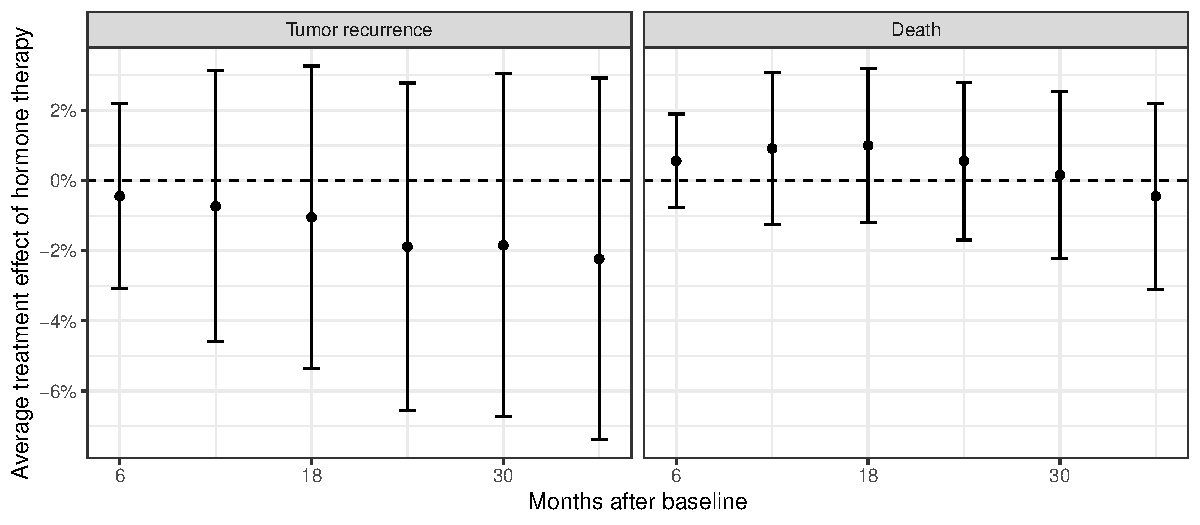
\includegraphics[width=.9\linewidth]{zelefsky-data-target-par.pdf}
\end{center}
\end{document}